\section{Clasificación de opciones complejas}

Para poder clasficar opciones más complejas, es útil observar las siguientes características: \textbf{dependencia del tiempo, flujo de dinero, dependencia del camino, dimensionalidad, orden y decisiones integradas}. Estas características darán información del método de fijación de precios se debe usar, si se puede usar código antiguo, cuanto tiempo se tardará en codificarlo y con qué velocidad se ejecutará.
\begin{figure}[H]
    \centering
    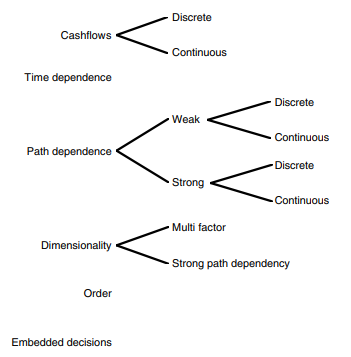
\includegraphics[width=0.65\linewidth]{Imagenes/Parte2/17_Clas_exot_path_ops/Clasif_Opt.png}
    \caption{Clasificación de opciones}
\end{figure}



\subsection{Dependencia del tiempo}
Referido a si se puede ejercer el derecho de compra o venta en cualquier momento, en ciertas fechas específicas o solo a tiempo de vencimiento. Es importante a la hora de hacer simulaciones porque por ejemplo si la opcion es tipo Bermuda, en la discretización del tiempo debe estar ese instante concreto.


\subsection{Flujo de dinero}
Se tiene que el contrato paga al propietario una cantidad fija $q$ en tiempo $t_0$, entonces se debe imponer una \textbf{condición de salto} para evitar arbitraje que, ignorando la dependencia del suyacente (como si fuese un bono con cupones), es:
\[
    \boxed{V(t_o^-) = V(t_o^+) + q}
\]
\begin{figure}[H]
    \centering
    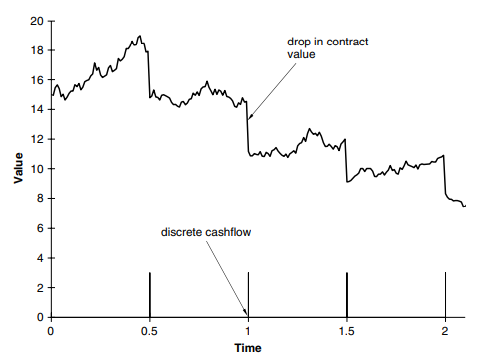
\includegraphics[width=0.65\linewidth]{Imagenes/Parte2/17_Clas_exot_path_ops/Jump_Condition.png}
    \caption{Condición de salto}
\end{figure}

Si el contrato depende de un subyacente ($V(S,t)$), entonces el flujo de dinero dependería del subyacente $q(S)$.

Si el flujo no fuese determinista (p.e.\ se lanza una moneda y se paga solo si sale cara), es más complejo y no se puede apelar al arbitraje. Se puede, por ejemplo, decir que la condición de salto sería que el cambio en el valor del contrato fuera el valor \textit{esperado} del flujo de caja
\[
    V(t_o^-) = V(t_o^+) + \mathbb{E}[q]
\]
pero esto tiene un riesgo.

Hasta aquí se ha hablado de pagos discretos, pero también podría haber pagos continuos, que son mucho más sencillos de incluir en el modelo y simplemente modifican la EDP.





\subsection{Dependencia del camino}
El payoff no solo depende del valor del subyacente a timepo de vencimiento, si no de todo el camino que ha recorrido.


\subsubsection{Strong Path Dependence}
Dependen de alguna propiedad del camino que ha recorrido el subyacente, por lo que tiene al menos una variable de dependencia extra y no se pueden definir como $V(S,t)$. Un ejemplo son las opciones asiáticas, que dependen del promedio del subyacente a lo largo del tiempo. En este caso, las variables independientes son el subyacente, el tiempo y el promedio del subyacente a lo largo del tiempo ($V(S,t,\overline{S})$).

Existen dos tipos de contratos así, los \textbf{discretely sampled} y los \textbf{continuously sampled} dependiendo de si el promedio se calcula en puntos discretos o continuamente. 

Una fuerte dependencia del camino implica que se debe trabajar en dimensiones superiores. Como consecuencia, el código puede tardar más en ejecutarse.


\subsubsection{Weak Path Dependence}
Tiene una cierta dependencia si ocurre cierto evento en el camino, pero no es necesario que se conozca todo el camino. Un ejemplo son las opciones barrier, que dependen de si el subyacente ha alcanzado cierto nivel. En este caso, las variables independientes solo son el subyacente y el tiempo ($V(S,t)$), pero se debe tener en cuenta si ha alcanzado cierto nivel o no. De nuevo, existen discretos y continuos, dependiendo de si se mira el subyacente en puntos discretos o continuamente.

A diferencia de las strong path dependence, estas opciones no necesitan trabajar en dimensiones superiores, por lo que el código puede ser más rápido y sencillo de implementar.






\subsection{Dimensionalidad}
Se refiere al número de variables independientes que tiene el contrato. Por ejemplo, para opciones vainilla europeas u opciones barrera las variables aleatorios son dos: subyacente y activo.

Dentro de los contratos con tres variables independientes se distinguen dos tipo:
\begin{itemize}
    \item Opciones en las que la varible extra es una medida de la trayectoria. Un ejemplo sería las opciones con una strong path dependence.
    \item Opciones en las que existe una segunda fuente de incertidumbre. Un ejemplo sería una opción sobre el máximo entre dos activos.
\end{itemize}


Computacionalmente, dimensiones mayores suponen tiempos de ejecución mayores. El número de dimensiones también indica qué tipo de método numérico utilizar. Para un número alto de dimensiones es útil usar Monte Carlo; para un número bajo es útil usar diferencias finitas.





\subsection{Orden}
Se puede expresar como la cantidad de opciones y por lo tanto de complejidad del contrato. Por ejemplo, los contratos de primer orden son aquellos sencillos como las vainilla europeas o incluso alguna opción dependientes del camino que solo dependan del camino del subyacente. 

Ordenes superiores son aquellos que dependen de otras opciones. Un ejemplo es la opción compuesta, p.e.\ una opción call que da derecho a comprar una put. La opción compuesta tiene una fecha de vencimiento $T_1$ y la opción subyacente tiene una fecha de vencimiento $T_2$.

Cuando una opción es de segundo orden o superior, primero se debe resolver la opción de primer orden. Por lo tanto, se debe trabajar a capas; primero los niveles inferiores y los resultados de estos se aplican a los niveles superiores. Esto significa que, computacionalmente, se debe resolver más de un problema para determinar el precio de la opción.





\subsection{Decisiones integradas}
El ejemplo más típico es el de las opciones americanas, que permiten ejercer el derecho de compra o venta en cualquier momento. 

Otro ejemplo son las passport option, en las que se compra y vende un activo: si a vencimiento hay beneficios se obtiene ese dinero y si no el contrato se cancela. Las decisiones en este caso son cuándo y cómo comprar y vender el activo.

Cuando un contrato incorpora decisiones, se necesita un algoritmo para determinar cómo se tomará esa decisión. Este algoritmo supone que el tenedor del contrato actúa para que el valor de la opción sea lo más alto posible para el emisor de la cobertura. El algoritmo de fijación de precios consiste entonces en buscar, entre todas las posibles estrategias de decisión del tenedor, la que maximice el valor de la opción.

Este tipo de opciones suelen suponer usar diferencias finitas en el código, y contendrá alguna línea en la que se busque el mejor precio, por lo que se debe tener cuidado con $\leq$ y $\geq$.







\section{Algunos ejemplos de derivados exóticos y dependientes del camino}

\subsection{Compounds options}
Las \textbf{compound options} son opciones sobre opciones, da la opción al poseedor de comprar (call) o vender (put) otra opción. Sea $F(S)$ el payoff de la opción subyacente a tiempo de vencimiento $T$, y sea $T_{C_0} < T$ la fecha de vencimiento de la opción compuesta en la que se obtiene $G(V(S,T_{C_0}))$ donde $V(S,t)$ es el valor de la opción subyacente. El primer paso es obtener el valor de la opción subyacente $V(S,t)$ que satisface:
\[
    \boxed{
        \left\{
        \begin{aligned}
            &\frac{\partial V}{\partial t} + \frac{1}{2}\sigma^2 S^2 \frac{\partial^2 V}{\partial S^2} + r S \frac{\partial V}{\partial S} - r V = 0 \\
            &V(S,T) = F(S)
        \end{aligned}
        \right.
    }
\]
Resolviendo se puede obtener $V(S,T_{C_0})$, que es el valor teórico de la opción subyacente a tiempo de vencimiento de la opción compuesta. A continuación se debe obtener el valor de la opción compuesta $C_0(S,t)$, que satisface:
\[
    \boxed{
        \left\{
        \begin{aligned}
            &\frac{\partial C_0}{\partial t} + \frac{1}{2}\sigma^2 S^2 \frac{\partial^2 C_0}{\partial S^2} + r S \frac{\partial C_0}{\partial S} - r C_0 = 0 \\
            &C_0(S,T_{C_0}) = G(V(S,T_{C_0}))
        \end{aligned}
        \right.
    }
\]

Por ejemplo, si se tiene una call sobre una call con strikes de $E$ para el subyacente y $E_{C_0}$ para la compuesta, los payoffs son:
\begin{align*}
    F(S) &= \max(S - E, 0) \\
    G(V) &= \max(V - E_{C_0}, 0)
\end{align*}




\subsection{Choosers options}
Las \textbf{chooser options} son parecidas a las compound, pero dan al poseedor la opción de elegir si quiere una call o una put como subyacente. Luego se quiere obtener el valor de la opción chooser $C_h(S,t)$ a partir del valor de las opciones subyacentes $V_1(S,t)$ y $V_2(S,t)$. Se cumple que:
\[
    \boxed{
        \begin{aligned}
            &\text{Call subyacente:} \quad
            \begin{cases}
                \dfrac{\partial V_1}{\partial t} + \dfrac{1}{2}\sigma^2 S^2 \dfrac{\partial^2 V_1}{\partial S^2} + r S \dfrac{\partial V_1}{\partial S} - r V_1 = 0 \\
                V_1(S, T) = \max(S - E_1, 0)
            \end{cases} \\[2ex]
            &\text{Put subyacente:} \quad
            \begin{cases}
                \dfrac{\partial V_2}{\partial t} + \dfrac{1}{2}\sigma^2 S^2 \dfrac{\partial^2 V_2}{\partial S^2} + r S \dfrac{\partial V_2}{\partial S} - r V_2 = 0 \\
                V_2(S, T) = \max(E_2 - S, 0)
            \end{cases} \\[2ex]
            &\text{Opción chooser:} \quad
            \begin{cases}
                \dfrac{\partial C_h}{\partial t} + \dfrac{1}{2}\sigma^2 S^2 \dfrac{\partial^2 C_h}{\partial S^2} + r S \dfrac{\partial C_h}{\partial S} - r C_h = 0 \\
                C_h(S, T_{C_h}) = \max\big(V_1(S, T_{C_h}) - E_1,\; V_2(S, T_{C_h}) - E_2,\; 0\big)
            \end{cases}
        \end{aligned}
    }
\]



\subsection{Extendible options}
Parecidas a las compound y choosers, pero en ciertos tiempos específicos, el poseedor elige entre aceptar el payoff original o extender el tiempo del contrato o incluso cambiar el strike.





\subsection{Range Notes}\label{sec:clas_range_notes}
Se suele aplicar sobre acciones, divisas o productos de renta fija. En su forma más básica, se paga una tasa $L$ siempre que el subyacente esté en un rango $S_l \leq S \leq S_u$ i.e.\ por cada $dt$ del subyacente que esté dentro del rango, se paga $L dt$. Se define $\mathcal{I}(S)$ como una función que toma el valor 1 si $S_l \leq S \leq S_u$ y 0 en caso contrario. Entonces, el range note satisface:
\[
    \boxed{\frac{\partial V}{\partial t} + \frac{1}{2}\sigma^2 S^2 \frac{\partial^2 V}{\partial S^2} + r S \frac{\partial V}{\partial S} - r V + L \mathcal{I}(S) = 0}
\]

Pueden existir variantes más complejas.



\subsection{Barrier Options}
El valor de una \textbf{barrier option} depende de si el subyacente alcanza cierto nivel llamado barrera.

Existen dos variedades principales:
\begin{itemize}
    \item \textbf{Knock-in}: se activan si el subyacente alcanza la barrera.
    \item \textbf{Knock-out}: se desactivan si el subyacente alcanza la barrera.
\end{itemize}

Siguen la ecuación clásica de Black-Scholes con una condición frontera especial. Se verá en profundidad en la sección~\ref{sec:barrier_options}.





\subsection{Asian Options}
El valor de una \textbf{Asian option} depende del promedio del subyacente a lo largo del tiempo. Se ven más adelante en la sección~\ref{sec:asian_options}.



\subsection{Lookback Options}
Las \textbf{lookback options} son opciones cuyo valor depende del máximo o mínimo del subyacente a lo largo del tiempo. Se verán más adelante en la sección~\ref{sec:lookback_options}.








\section{Resumen de la clasificación}
\begin{table}[H]
    \centering
    \begin{tabularx}{\linewidth}{|X|X|X|}
        \hline
        \textbf{Clasificación} & \textbf{Ejemplos} & \textbf{Consecuencias} \\
        \hline
        Dependencia del tiempo & Bermudan, ejercicio discreto, muestreo discreto, \ldots & Hay que llevar la cuenta del tiempo en el código \\
        \hline
        Flujo de dinero & Swap, pagos, \ldots & Salto en el valor de la opción / Término fuente en la EDP \\
        \hline
        Dependencia del camino & Barrera, asiática, lookback, \ldots & Si la dependencia del camino es fuerte, se necesita una dimensión extra \\
        \hline
        Dimensión & Muy dependiente del camino, multi-activo, \ldots & Monte Carlo puede ser mejor que diferencias finitas \\
        \hline
        Orden & Compuestas, en barreras, \ldots & Resolver primero las opciones de nivel inferior e introducir el resultado en el nivel superior \\
        \hline
        Decisiones & Americana, passport, chooser, \ldots & Diferencias finitas mejor que Monte Carlo, ‘optimizar’ \\
        \hline
    \end{tabularx}
    \caption{Implicaciones de la clasificación de derivados}
\end{table}


\begin{table}[H]
    \centering
    \begin{tabularx}{\linewidth}{|X|X|X|X|X|X|X|}
        \hline
        & \textbf{Depend.\ tiempo} & \textbf{Flujo dinero} & \textbf{Depend.\ camino} & \textbf{Dimensión} & \textbf{Orden} & \textbf{Decisiones} \\
        \hline
        \textbf{Compund/ Chooser} & No & No & Weak & 2 & Segundo & No \\
        \hline
        \textbf{Range Notes} & No & Sí (continuo) & Weak & 2 & Primero & No \\
        \hline
        \textbf{Barrier Options} & No & No & Weak & 2 & Primero (Knock-Out)/ Segundo (Knock-In) & No \\
        \hline
        \textbf{Asian Options} & Si (discreto)/ No (continuo) & No & Strong & 3 & Primero & No \\
        \hline
        \textbf{Lookback Options} & Si (discreto)/ No (continuo) & No & Strong & 3 & Primero & No \\
        \hline
        \textbf{Passport Options} & No & No & Weak & 3 & Primero & Si \\
        \hline
        \textbf{Forward-start Options} & No & No & Weak & 2 & Segundo & No \\
        \hline
        \textbf{Shout Options} & No & No & Strong & 3 & Primero & Yes \\
        \hline
        \textbf{Volatility Options} & Si & No & Strong (discreto) & 4 & Primero & No \\
        \hline
        \textbf{Parisian Options} & No & No & Strong (continuo) & 3 & Primero(Out)/ Segundo?(In) & No \\
        \hline
    \end{tabularx}
    \caption{Clasificación de derivados}
\end{table}








